\documentclass[letterpaper]{article}
\usepackage[margin=1in]{geometry}
\usepackage[utf8]{inputenc}
\usepackage{textcomp}
\usepackage{amssymb}
\usepackage{natbib}
\usepackage{graphicx}
\usepackage{gensymb}
\usepackage{amsthm, amsmath, mathtools}
\usepackage[dvipsnames]{xcolor}
\usepackage{enumerate}
\usepackage{mdframed}
\usepackage[most]{tcolorbox}
\usepackage{csquotes}
% https://tex.stackexchange.com/questions/13506/how-to-continue-the-framed-text-box-on-multiple-pages

\tcbuselibrary{theorems}

\newcommand{\R}{\mathbb{R}}
\newcommand{\Z}{\mathbb{Z}}
\newcommand{\N}{\mathbb{N}}
\newcommand{\Q}{\mathbb{Q}}
\newcommand{\C}{\mathbb{C}}
\newcommand{\code}[1]{\texttt{#1}}
\newcommand{\mdiamond}{$\diamondsuit$}
\newcommand{\PowerSet}{\mathcal{P}}
\newcommand{\Mod}[1]{\ (\mathrm{mod}\ #1)}
\DeclareMathOperator{\lcm}{lcm}

%\newtheorem*{theorem}{Theorem}
%\newtheorem*{definition}{Definition}
%\newtheorem*{corollary}{Corollary}
%\newtheorem*{lemma}{Lemma}
\newtheorem*{proposition}{Proposition}


\newtcbtheorem[number within=section]{theorem}{Theorem}
{colback=green!5,colframe=green!35!black,fonttitle=\bfseries}{th}

\newtcbtheorem[number within=section]{definition}{Definition}
{colback=blue!5,colframe=blue!35!black,fonttitle=\bfseries}{def}

\newtcbtheorem[number within=section]{corollary}{Corollary}
{colback=yellow!5,colframe=yellow!35!black,fonttitle=\bfseries}{cor}

\newtcbtheorem[number within=section]{lemma}{Lemma}
{colback=red!5,colframe=red!35!black,fonttitle=\bfseries}{lem}

\newtcbtheorem[number within=section]{example}{Example}
{colback=white!5,colframe=white!35!black,fonttitle=\bfseries}{def}

\newtcbtheorem[number within=section]{note}{Important Note}{
        enhanced,
        sharp corners,
        attach boxed title to top left={
            xshift=-1mm,
            yshift=-5mm,
            yshifttext=-1mm
        },
        top=1.5em,
        colback=white,
        colframe=black,
        fonttitle=\bfseries,
        boxed title style={
            sharp corners,
            size=small,
            colback=red!75!black,
            colframe=red!75!black,
        } 
    }{impnote}
\usepackage[utf8]{inputenc}
\usepackage[english]{babel}
\usepackage{fancyhdr}
\usepackage[hidelinks]{hyperref}

\pagestyle{fancy}
\fancyhf{}
\rhead{Math 103A}
\chead{June 29th, 2021}
\lhead{Course Notes}
\rfoot{\thepage}

\setlength{\parindent}{0pt}

\begin{document}

\begin{titlepage}
    \begin{center}
        \vspace*{1cm}
            
        \Huge
        \textbf{Math 103 Notes}
            
        \vspace{0.5cm}
        \LARGE
        Modern Algebra
            
        \vspace{1.5cm}
            
        \vfill
            
        Summer Session 1 2021\\
        Taught by Professor Kyle Meyer
    \end{center}
\end{titlepage}

\pagenumbering{gobble}

\newpage 

\begingroup
    \renewcommand\contentsname{Table of Contents}
    \tableofcontents
\endgroup

\newpage
\pagenumbering{arabic}

\section{Review: Equivalence Relations}
We will go over topics covered in other courses that will be used in this course. We begin with the topic of equivalence relations. 

\subsection{Equivalence Relations}
Let $X$ be a non-empty set. Then, a \textbf{relation} over $X$ is a subset $R$ of $X \times X$. If $(x, y) \in R$, we say that $x$ is $R$-related to $y$ and write $x R y$. 

\bigskip 

So, for these relations, we should think about inequalities equalities, or congruences between integers. 

\bigskip 

Suppose $R$ is a relation over $X$. Then:
\begin{itemize}
    \item $R$ is called \textbf{reflexive} if $\forall x \in X$, $x R x$. That is, every $x \in X$ is related to itself. 
    \item $R$ is called \textbf{symmetric} if $\forall x, y \in X$, $x R y \implies y R x$. In other words, if $x$ is related to $y$, is $y$ related to $x$? 
    \item $R$ is called \textbf{transitive} if $\forall x, y, z \in X$, $x R y$ and $y R z$ implies that $x R z$. 
\end{itemize}

\begin{definition}{Equivalence Relation}{equivRel}
    $R$ is called an \textbf{equivalence relation} if $R$ is reflexive, symmetric, and transitive. 
\end{definition}

\textbf{Remark:} An equivalence relation is essentially an equality with respect to a certain measurement. In life, we often measure things or people with respect to properties (for example, scores or ratings). So, when we want to compare things, we pick a certain property and then, \emph{from that point of view}, determine whether these things are equal. In this regard, equivalence relations are exactly equalities. 

\subsubsection{Example: Relations}
Suppose $X$ and $Y$ are two non-empty sets and $f: X \to Y$ is a function. Let $\sim$ be the following relation over $X$:
\[\forall x_1, x_2 \in X \quad x_1 \sim x_2 \iff f(x_1) = f(x_2)\]
Then, $\sim$ is an equivalence relation\footnote{Another way of interpreting this statement is as follows: $x_1$ is in relation to $x_2$ precisely when $f(x_1) = f(x_2)$. The claim here, then, is that this is an equivalence relation.}.

\begin{proof}
    We determine if an relation is an equivalence relation if it satisfies the three properties mentioned above.
    \begin{itemize}
        \item \underline{Reflexivity:}
        \[\forall x \in X, f(x) = f(x) \implies x \sim x\]

        \item \underline{Symmetric:}
        \[x_1 \sim x_2 \implies f(x_1) = f(x_2) \implies f(x_2) = f(x_1) \implies x_2 \sim x_1\]

        \item \underline{Transitive:}
        We know that:
        \[\forall x_1, x_2 \in X \qquad x_1 \sim x_2 \implies f(x_1) = f(x_2)\]
        We also know that:
        \[\forall x_2, x_3 \in X \qquad x_2 \sim x_3 \implies f(x_2) = f(x_3)\]
        It follows that if $f(x_1) = f(x_2)$ and $f(x_2) = f(x_3)$, then $f(x_1) = f(x_3)$ and thus, $x_1 = x_3$. Namely, $x_1 \sim x_2$ and $x_2 \sim x_3$, then $x_1 \sim x_3$. 
    \end{itemize}
    It follows that this is an equivalence relation. 
\end{proof}

\subsection{Equivalence Relation Partitions}
Recall that $P$ is called a \textbf{partition} of a non-empty set $X$ if:
\begin{itemize}
    \item \underline{Subsets:} $P$ consists of non-empty subsets of $X$. 
    \item \underline{Disjointness:} $A, B \in P$ and $A \neq B \implies A \cap B = \emptyset$. In other words, the subsets are disjoint. 
    \item \underline{Covering:} $\forall x \in X$, $\exists A \in P$ such that $x \in A$. In other words, every element in $X$ will be in one of the subsets. Alternatively, $\bigcup_{A \in P} A = X$. 
\end{itemize}

\textbf{Remark:}
\begin{itemize}
    \item As mentioned, $P$ is a set of sets. For instance, if we have $X = \{1, 2, 3\}$, one possible $P$ is $P = \{\{1\}, \{2, 3\}\}$.
    \item Below is a visual diagram of what a partition may look like.
\end{itemize}
\begin{center}
    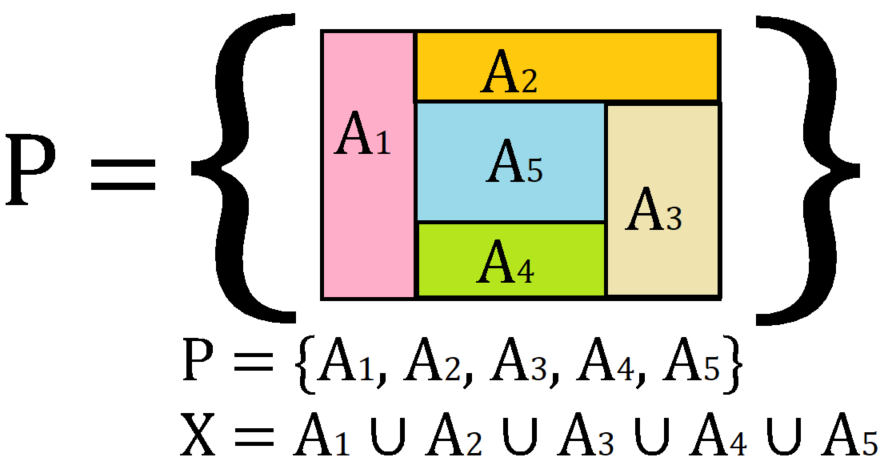
\includegraphics[scale=0.4]{img/partition.PNG}
\end{center}

Suppose $P$ is a partition of $X$. Then, we can get a classification function from $X$ to $P$:
\[X \to P\]
\[x \mapsto [x]_P\]
Here, $[x]_P$ is the unique element of $P$ which contains $x$. In other words, if we refer to the above diagram, we can think of $[x]_P$, a set, as one of the sets $A_1$, $A_2$, $A_3$, $A_4$, or $A_5$ which contains $x$. So, we can think of this function as saying that every $x \in X$ belongs to one of the sets $[x]_P$. 

\bigskip 

Notice that, because of the \textbf{covering} condition, $x$ is contained in some element of $P$; additionally, because of the \textbf{disjointness} condition, $x$ is in an unique element of $P$ (i.e. it is in \underline{one} of the sets which is in $P$). So, it follows that the function is well-defined. 

\bigskip 

By the previous example, $x \sim_P y \iff [x]_P = [y]_P$ is an equivalence relation. So, we obtain the following lemma. 
\begin{lemma}{}{}
    Suppose $P$ is a partition of a non-empty set $X$. For $x, y \in X$, $x \sim y$ if $x$ and $y$ are in the same element of $P$. Then, $\sim$ is an equivalence relation.
\end{lemma}
\textbf{Remark:} Essentially, what this lemma is saying is that if $x \sim y$, then both $x$ and $y$ are in the same set which is in $P$. In other words, if we refer to the above diagram again, we can think of this situation as saying that both $x$ and $y$ are in \underline{one} of $A_1$, $A_2$, $A_3$, $A_4$, or $A_5$. The diagram below complements the proof.

\begin{center}
    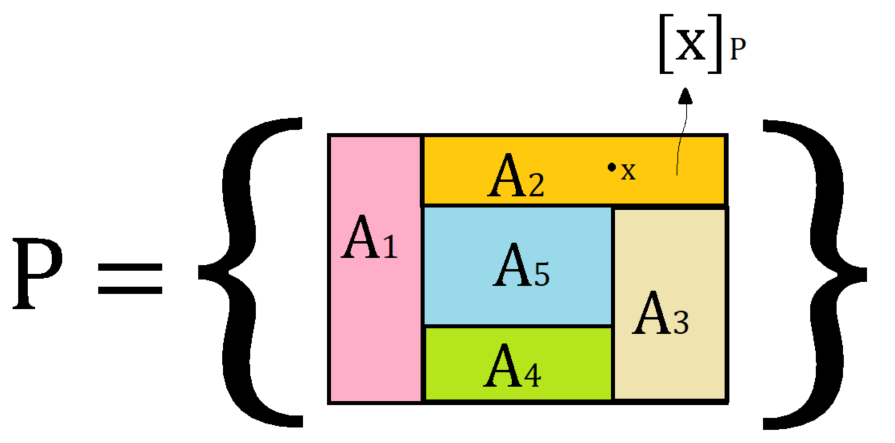
\includegraphics[scale=0.30]{img/partition_x.PNG}
\end{center}

\begin{proof}
    For $x \in X$, let $[x]_P$ to be the unique element of $P$ which contains $x$. So, $x \mapsto [x]_P$ is a function from $X \to P$. By the previous example, $x \sim y \iff [x]_p = [y]_p$ is an equivalence relation over $X$. Notice that this means $x \sim y$ exactly when $x$ and $y$ are in the same element of $P$. 
\end{proof}

\subsection{Equivalence Relation Classes}
Now, suppose that $\sim$ is the equivalence relation over a non-empty set $X$, we can partition $X$ with respect to $\sim$. 

\bigskip 

For $x \in X$, we let $[x] = \{y \in X \mid y \sim x\}$ (all the elements that are $\sim$-related to $x$).\footnote{So, it's obvious that $[x] \subseteq X$.} We call $[x]$ the \textbf{equivalence class of $x$ with respect to $\sim$}. When $x \sim y$, we can say that $x$ is equivalent to $y$ with respect to $\sim$. 

\begin{proposition}
    Suppose $\sim$ is an equivalence relation over a non-empty set $X$. Then, $\{[x] \mid x \in X\}$ is a partition of $X$. 
\end{proposition}
This proposition is essentially asking us to show the following properties: 
\begin{itemize}
    \item Covering: Every element of this set belongs to one of these equivalence classes. 
    \item Disjointness: If we pick two equivalence classes, they do not intersect.
\end{itemize}
The following lemma follows from this proposition.
\begin{lemma}{}{}
    \[x \sim y \iff [x] = [y]\]
\end{lemma}
\begin{proof}
    We want to show that $[x] = [y] \implies x \sim y$. Recall that the equivalence class of $x$ ($[x]$) and the equivalence class of $y$ ($[y]$) are \emph{sets} and, in particular, we know that $[x]$ consists of all elements that are related to $x$, including $x$. Since $\sim$ is reflexive, we know that:
    \[x \sim x \implies x \in [x]\]
    But, since $[x] = [y]$, then it follows that $x \in [y] \implies x \sim y$. Thus, $[x] = [y] \implies x \sim y$. 
    
    \bigskip 

    To show that $x \sim y \implies [x] = [y]$, we need to show equality of sets $[x] = [y]$. This means that it is necessary and sufficient to prove $[x] \subseteq [y]$ and $[y] \subseteq [x]$.
    \begin{itemize}
        \item To prove $[x] \subseteq [y]$, we let $z \in [x]$. This means that $z \sim x$. However, since $x \sim y$, by transitivity, it follows that $y \sim z$, which implies that $z \in [y]$. Hence, $[x] \subseteq [y]$. 
        \item We note that $x \sim y \implies y \sim x$ by symmetry. Therefore, by the first bullet point, $[y] \subseteq [x]$.
    \end{itemize} 
    So, it follows that $x \sim y \implies [x] = [y]$. 
\end{proof}

Now that we proved the lemma, we can now prove the proposition. 
\begin{proof}
    As mentioned, we need to show that the covering and disjointness properties exist in this partition.
    \begin{itemize}
        \item \underline{Covering:} $\forall x \in X$, we know that $x \sim x$ by the reflexive property (since $\sim$ is an equivalence relation). Thus, it follows that $x \in [x]$. This means that $x$ is related to $x$ and $x$ is an equivalence class of $x$, so every element in $X$ belongs to one of the equivalence classes. This implies that the $[x]$ sets are non-empty subsets and cover $X$.
        \item \underline{Disjointness:} Suppose $z \in [x] \cap [y]$ (both equivalence classes are not disjoint). We need to show that they are equal. We know that:
        \[z \in [x] \cap [y] \implies z \in [x] \implies z \sim x \implies [z] = [x]\]
        \[z \in [x] \cap [y] \implies z \in [y] \implies z \sim y \implies [z] = [y]\]
        Where the last two steps came from the lemma. Then, putting these two together, we have:
        \[[z] = [x] \text{ and } [z] = [y] \implies [x] = [y]\]
        We showed that $[x] \cap [y] \neq \emptyset \implies [x] = [y]$, the contrapositive of the disjointness property. 
    \end{itemize}
    Thus, the proof is complete. 
\end{proof}

\subsection{Summary}
The following diagram provides a brief summary of what we've learned\footnote{This diagram was taken from Professor Alireza Salehi Golsefidy's notes.}
\begin{center}
    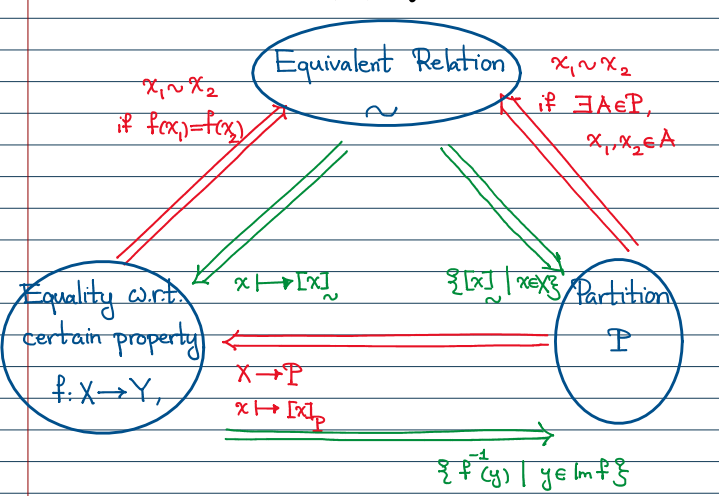
\includegraphics[scale=0.9]{img/equiv_relation.PNG}
\end{center}








% --------------------------------------------------------- %
%                   NEW SECTION                             %
% --------------------------------------------------------- %
\newpage 
\section{Review: Congruences, Long Division, Modulo}
In this section, we discuss congruences, long division, and modulo. 

\subsection{Congruence}
The set of integers is denoted by $\Z$. For $a, b \in \Z$, we say that $a$ divides $b$ and write $a | b$ if $b = ak$ for some $k \in \Z$. Suppose $n$ is a non-zero integer. Then, we say that $a$ is \textbf{congruent} to $b$ modulo $n$ and write one of the following if $n | (a - b)$:
\[a \equiv b \Mod{n}\]
\[a \overset{n}{\equiv} b\]
One way to think of this is through a clock. A clock has $n$ numbers (usually 12 numbers). Then, $a$ and $b$ will be on the same spot. For instance, suppose we have 9PM (denoted by the 21st hour). Then, we know that:
\[21 \equiv \boxed{9} \Mod{12}\]
In other words, the hour hand for 9PM will be in the same position as 9AM. 

\subsection{Congruence and Equivalence Relations}
\begin{lemma}{}{}
    $\overset{n}{\equiv}$ is an equivalence relation over $\Z$. 
\end{lemma}
\begin{proof}
    Recall that something is an equivalence relation if it satisfies the three properties mentioned in definition \ref{def:equivRel}. So, we need to show that $\overset{n}{\equiv}$ satisfies these. 
    \begin{itemize}
        \item \underline{Reflexive}: For every $a \in \Z$, we know that $a - a = 0$ is a multiple of $n$ as $n \cdot 0 = 0$. Hence, $a \overset{n}{\equiv} a$. 
        \item \underline{Symmetric}: We have that: 
        \begin{equation*}
            \begin{aligned}
                a \overset{n}{\equiv} b &\implies n | (a - b) \\ 
                    &\implies \exists k \in \Z, a - b = nk \\ 
                    &\implies b - a = n\underbrace{(-k)}_{\text{In } \Z} \\ 
                    &\implies b \overset{n}{\equiv} a
            \end{aligned}
        \end{equation*}

        \item \underline{Transitive:} We know that:
        \[a \overset{n}{\equiv} b \implies n | (a - b) \implies \exists k \in Z, a - b = nk\]
        We also know that:
        \[b \overset{n}{\equiv} c \implies n | (b - c) \implies \exists l \in \Z, b - c = nl\]
        Combining the statements, we now have:
        \[(a - b) + (b - c) = nk + nl \implies a - c = n\underbrace{(k + l)}_{\text{In } \Z} \implies a \overset{n}{\equiv} c\]
    \end{itemize}
    Thus, $\overset{n}{\equiv}$ is an equivalence class. 
\end{proof}

\subsection{Congruence and Partitions}
As we have seen earlier, every equivalence relation gives us a \textbf{partition} and an \textbf{equality function}. For $a \in \Z$, the equivalence class of $a$ with respect to $\overset{n}{\equiv}$ is called the \textbf{mod-$n$ residue class of $a$} and is denoted by $[a]_n$. By the results that we proved for equivalence relations, we have that:
\begin{itemize}
    \item $\{[a]_n \mid a \in \Z\}$ is a partition of $\Z$; and 
    \item $a \overset{n}{\equiv} b \iff [a]_n = [b]_n$ 
\end{itemize}

The partition $\{[a]_n \mid a \in \Z\}$ is denoted by $\Z_n$ and it is called \textbf{the set of integers modulo $n$}. Notice that:
\begin{equation*}
    \begin{aligned}
        b \in [a]_n &\iff b \overset{n}{\equiv} a \\ 
            &\iff n | (b - a) \\ 
            &\iff \exists k \in \Z, b - a = nk \\ 
            &\iff \exists k \in \Z, b = a + nk \\ 
            &\iff b \in \{a + nk \mid k \in \Z\} & \text{Arithmetic Progression}
    \end{aligned}
\end{equation*} 

To understand the set $\Z_n$ better, we recall the well-ordering principle and the long division property of integers. One of the important properties of positive integers is the \textbf{well-ordering principle}. This principle can be viewed as an axiom that we assume $\Z$ has. 

\subsubsection{Well-Ordering Principle}
Every non-empty subset of the set $\Z_{\geq 0}$ of non-negative integers has a minimum. Using the well-ordering principle, we can prove the division algorithm. 

\subsubsection{The Division Algorithm}
For every $a \in \Z$, $b \in \Z - \{0\}$, there is a unique pair $(q, r)$ of integers such that:
\[a = bq + r \qquad 0 \leq r \leq |b|\]
To show that this is the case, consider the following diagram:
\begin{center}
    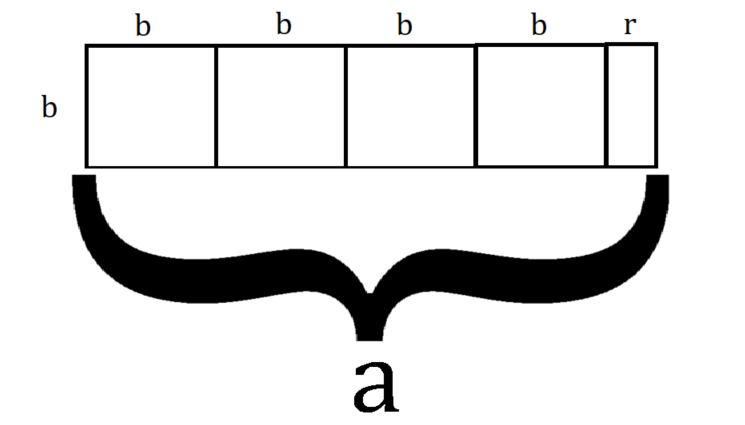
\includegraphics[scale=0.4]{img/mod_div.PNG}
\end{center}
For positive integers $a$ and $b$, we can keep ``cutting off'' the $b \times b$ squares until we are left with either a rectangle smaller than $b \times b$ (i.e. if $r > 0$), or nothing at all (i.e. $r = 0$). In this sense, the number of $b \times b$ squares that we cut off is denoted by $q$ (or $k$ soon). Then, it follows that $r$ is the smallest non-negative integer in the arithmetic progression $a - bk$.

\bigskip 

Now, we want to formalize this argument. We begin by defining: 
\[\Sigma := [a]_b \cap \Z_{\geq 0} = \{a + bk \mid k \in \Z, a + bk \geq 0\}\]
Here, we denote $\Sigma$ as a variable, not a summation. We want to use the well-ordering principle on the set $\Sigma$ to show that it has a minimium (more specifically, that $\Sigma$ is not empty). Our first claim is:
\[\Sigma \text{ is not empty.}\]
\begin{proof}
    Since $b \neq 0$, we know that $|b| \geq 1$. Hence, $|b||a| \geq |a|$. Therefore:
    \[\underbrace{|b|(|a| + 1) + a}_{a \pm b(|a| + 1)} \geq |a| + |b| + a \geq |b| > 0\]
    It follows that $[a]_b$ has a positive integer. 
\end{proof}
By the above claim and the well-ordering principle, $\Sigma$ has a minimum. Now, suppose $r$ is the minimum of $\Sigma$. Then, $r = a - bq$ for some $q \in \Z$. Our second claim is:
\[r < |b|\]
\begin{proof}
    Suppose to the contrary that $r \geq |b|$. Then, $r - |b| \geq 0$ and:
    \[r - |b| = a - bq - |b| = a - b(q \pm 1)\]
    In the above statement, we know that $r = a - bq$, which is in the arithmetic progression. When we subtract $|b|$, we are still in this arithmetic progression since all we're doing is adding or subtracting $b$; in either case, we're not leaving the arithmetic progression. So, it follows that $r - |b|$ is still in this arithmetic progression.

    \bigskip 

    Hence, $r - |b| \in \Sigma$ (recall that $\Sigma$ consists of non-negative integers). This is a contradiction as $r - |b|$ is smaller than the minimum $r$ of $\Sigma$. 
\end{proof}
By this claim, we obtain the existence of the pair $(q, r)$ with:
\begin{itemize}
    \item $a = bq + r$
    \item $0 \leq r < |b|$
\end{itemize}
Now, we want to prove the uniqueness.
\begin{proof}
    Suppose the pairs $(q, r)$ and $(q', r')$ satisfy the desired properties; that means:
    \begin{enumerate}[(a)]
        \item $a = bq + r = bq' + r'$
        \item $0 \leq r, r' \leq |b|$
    \end{enumerate}
    Then, $b(q - q') = (r' - r)$. Notice that:
    \[0 \leq r \implies r' - r \leq r' < |b|\]
    \[0 \leq r' \implies r' - r \geq -r > -|b|\]
    Then, we have that:
    \[|r' - r| < |b|\]
    And we obtain that:
    \[|r' - r| = |b|(q - q') = |b| |q - q'|\]
    And, thus:
    \[|b||q - q'| < |b|\]
    This implies that $|q - q'| < 1$. Since $|q - q'|$ is a non-negative integer less than 1, it is 0. Thus, $q = q'$. It follows that:
    \[r' - r = b(q - q') = 0\]
    This implies that $r = r'$. Thus, this shows the uniqueness. 
\end{proof}
Suppose the pair $(q, r)$ is given in the long division algorithm. Then, $q$ is called the \textbf{quotient} of $a$ divided by $b$ and $r$ is called the remainder of $a$ divided by $b$. Using the long division algorithm, we obtain that $\Z_n$ has $n$ elements. 

\begin{proposition}
    Suppose $n$ is an integer more than 1. Then:
    \[\Z_n = \{[0]_n, [1]_n, \dots, [n - 1]_n\} \quad |\Z_n| = n\]
\end{proposition}
\begin{proof}
    For every $a \in \Z$, by the long division algorithm, there are integers $q$ and $r$ such that $a = nq + r$ and $0 \leq r < n$. 
\end{proof}


% \overset{n}{\equiv}




% --------------------------------------------------------- %
%                   NEW SECTION                             %
% --------------------------------------------------------- %
\newpage 
\section{Binary Operations and Group Theory}
We want to explore the idea behind \emph{algebraic structures}. In particular, we want to explore these structures in more detail compared to earlier courses (either in past college or high school algebra classes).

\bigskip 

To do this, we need to think about \emph{what} algebra really is. We might think about solving equations like $x^2 + 3x + 5 = 0$ for $x$. In particular, what is really happening here?

\bigskip 

Well, there are a couple of operations going on. Specifically, we have \emph{addition} and \emph{multiplication}. 
\[x \cdot x + 3 \cdot x + 5 = 0\]
We now want to examine these operations. Both of these operations $(+, \cdot)$ take in \underline{two numbers} and output \underline{one number}. The question we might have, then, is: how can we can generalize these operations?

\subsection{Binary Operations}
A \textbf{binary operation} is a way of taking in two values and outputting one value. Of course, we might now ask: what can these values be? These values can come from any specific set. 

\bigskip 

For example, we can consider addition over the integers ($\Z$). The sum of two integers is an integer. Similarly, we could consider multiplication over the integers. Again, the product of two integers is an integer. We could also consider multiplication or addition over the real, rational, or complex numbers. 

\bigskip 

The idea is that whatever ``type'' we give our binary operation, we will get that same ``type'' for our output. To formalize this, we have the following definition:  
\begin{definition}{Binary Operation}{}
    A binary operation $*$ over a set $S$ is a function mapping $f: S \times S \to S$. For each $(a, b) \in S \times S$, we will denote the element $*((a, b))$ of $S$ by $a * b$.\footnote{As a side note, in this class, $a * b$ is equivalent to $f(a, b)$ and $b * a$ is equivalent to $f(b, a)$.}
\end{definition}
%Recall that the Cartesian Product of two sets $S_1$ and $S_2$ is denoted by $S_1 \times S_2$ and is defined by:
%\[S_1 \times S_2 = \{(s_1, s_2) \mid s_1 \in S_1, s_2 \in S_2\}\]
%Here, we note that $(a, b) \neq (b, a)$ unless $a = b$. 
%\bigskip 

We also introduce the notion of closure, which will be used later. 
\begin{definition}{Closure}{}
    Let $*$ be a binary operation on $S$ and let $H$ be a subset of $S$. The subset $H$ is \textbf{closed under} $*$ if for all $a, b \in H$ we also have $a * b \in H$. In this case, the binary operation on $H$ given by restricting $*$ to $H$ is the \textbf{induced operation} of $*$ on $H$.
\end{definition}

Anything that is ``like'' addition or multiplication is probably a binary operation. For example, let's consider \textbf{matrices}.
\begin{itemize}
    \item Addition of matrices of a fixed dimension. More specifically, the set of $n \times m$ matrices (here, $n$ and $m$ are fixed positive integers) over the integers, rationals, reals, or complex numbers under matrix addition is a binary operation.
    \[
        \begin{bmatrix}
            a_{11} & a_{12} & a_{13} \\ 
            a_{21} & a_{22} & a_{23}
        \end{bmatrix} + \begin{bmatrix}
            b_{11} & b_{12} & b_{13} \\ 
            b_{21} & b_{22} & b_{23}
        \end{bmatrix} = \begin{bmatrix}
            a_{11} + b_{11} & a_{12} + b_{12} & a_{13} + b_{13} \\ 
            a_{21} + b_{21} & a_{22} + b_{22} & a_{23} + b_{23}
        \end{bmatrix}
    \]

    \item Multiplication of matrices of a fixed dimension. More specifically, the set of $n \times n$ matrices (square matrices). We could also just multiply a $(n \times m)$ matrix by a $(k \times l)$ matrix assuming $m = k$ (otherwise, multiplying these two matrices will result in undefined behavior). 
\end{itemize}

So far, we considered binary operations on infinite sets in which we need some sort of formula to describe (e.g. $f_{\cup}(A, B) = A \cup B$). Now, if we have a finite set, we could define a binary operation exhaustively by just saying what the binary operation does on every pair of entries.

\bigskip 

For example, given the set $S = \{a, b, c, d, e\}$. We can define a binary operation on $S$ with the below (random) table (first entry on left side, second entry on top side). 
\begin{center}
    \begin{tabular}{c|c|c|c|c|c}
            & $a$ & $b$ & $c$ & $d$ & $e$ \\ 
        \hline 
        $a$ & $a$ & $c$ & $d$ & $d$ & $e$ \\ 
        $b$ & $b$ & $c$ & $c$ & $b$ & $a$ \\ 
        $c$ & $d$ & $e$ & $e$ & $b$ & $b$ \\ 
        $d$ & $a$ & $a$ & $a$ & $c$ & $a$ \\ 
        $e$ & $b$ & $b$ & $c$ & $c$ & $d$
    \end{tabular}
\end{center}
Denote the binary operation to be $\#$.
\begin{itemize}
    \item What is $c \# d$? The answer is $b$. 
    \item What is $e \# ((a \# b) \# c)$? The answer is $d$.
    \item Suppose we have $X \# a = a$. What is $X$? The answer is $X = a, d$.
\end{itemize}

\subsection{Properties of Binary Operations}
What properties could binary operations have?\footnote{In this course, we will consider binary operations with all the properties excluding commutativity.}

\begin{itemize}
    \item \textbf{Commutativity:} A binary operation is commutative if the order of the two inputs does not matter. For example, if $f$ is a function corresponding to a binary operation, then:
    \[f(a, b) = f(b, a) \quad \forall a, b \in S\] 
    More commonly:
    \[a * b = b * a \quad \forall a, b \in S\]

    For example, addition or multiplication of numbers is commutative. Unions and intersections of sets is also commutative. \emph{However}, matrix multiplication is \emph{not} commutative. Our example above is also not commutative. 

    \item \textbf{Associativity:} A binary operation is associative if the order of applying the operation (in a string) does not matter. Specifically:
    \[(a * b) * c = a * (b * c) \quad \forall a, b, c \in S\]
    Which means that we can write $a * b * c$ without ambiguity.
    
    \bigskip 

    For example, addition or multiplication of numbers is associative. Addition or multiplication of matrices is also associative. Our example above is not associative. 

    \item \textbf{Identity:} A binary operation has a two-sided identity element and a two-sided inverse for every element. 
    
    \bigskip 
    
    More specifically, we say that $\epsilon$ is a left identity if $f(\epsilon, s) = s$ for all $s \in S$. $\epsilon$ is a right identity if $f(s, \epsilon) = s$ for all $s \in S$. Then, $\epsilon$ is a two-sided identity if it is both a left identity and right identity.  
    
    \bigskip 

    For example, 0 is a two-sided identity for addition and 1 is a two-sided identity for multiplication. For matrix addition, the zero-matrix is a two-sided identity. For matrix multiplication, the matrix with ones on the diagonal and zeros everywhere else is the identity element. In our example above, $\#$ does not have a left or right identity. 

    \bigskip 

    Given a two-sided identity, we can also consider the idea of an inverse. In addition, this is the negative/negation. In multiplication, this is the reciprocal. The additive inverse of $x$ is $-x$. The multiplicative inverse of $x$ is $\frac{1}{x}$ (for all $x \neq 0$). 
    
    \bigskip 
    
    For a general binary operation $f: S \times S \to S$ with a two-sided identity $\epsilon$, an element $s \in S$ has a two-sided inverse if there exists an element $t \in S$ such that:
    \[\underbrace{f(s, t)}_{\text{Right Inverse}} = \overbrace{f(t, s)}^{\text{Left Inverse}} = \epsilon\] 

    So, a property for binary operations would be for every element to have a \underline{two-sided inverse}, which requires a \underline{two-sided identity element}.
\end{itemize}

\textbf{Remark:} Commutativity does not imply associativity.

\subsection{Groups}
Of course, the properties of binary operations that were discussed just now are very much applicable in something called \textbf{groups}. 

\begin{definition}{Group}{}
    A group is a set $G$, closed under a binary operation $*$, satisfying the three properties:
    \begin{enumerate}
        \item \underline{Associativity}: For all $a, b, c \in G$, we have:
        \[(a * b) * c = a * (b * c)\]

        \item \underline{Identity Element:} There is an element $\epsilon \in G$ such that for all $x \in G$:
        \[\epsilon * x = x * e = x\]

        \item \underline{Inverse:} Corresponding to each $a \in G$, there is an element $a' \in G$ such that:
        \[a * a' = a' * a = \epsilon\]
    \end{enumerate}
\end{definition}
\textbf{Remark:} Notationally, this can be represented by $(G, *)$ or $\langle G, * \rangle$. This is saying that we are pairing a set with a binary operation. 

\subsubsection{Example: Addition}
For example, the integers under addition are a group. Notationally, this is represented by $(\Z, +)$. 
\begin{itemize}
    \item It's obvious that addition is associative. That is:
    \[(a + b) + c = a + (b + c) = a + b + c\]

    \item The identity element is 0. This is because:
    \[0 + x = x + 0 = x\]

    \item The inverse is $-x$. This is because:
    \[x + (-x) = (-x) + x = 0\]
\end{itemize}
We also know that the reals, rationals, or complex numbers under addition are also groups. Notationally, this is represented by $(\R, +)$, $(\Q, +)$, or $(\C, +)$, respectively. 

\subsubsection{Example: Multiplication}
Let's now consider multiplication. In particular, multiplication does give a binary operation over $\Z$, $\Q$, $\R$, and $\C$. It's obvious that this is associative and 1 is the two-sided identity element. However, what about the inverse? 
\begin{itemize}
    \item If we try to take the integers under multiplication as a group, then we'll run into problems. This is because the multiplicative inverse of every \underline{integer} except $\pm 1$ is not an integer. For example, if we tried 2, then the multiplicative inverse of 2 is $\frac{1}{2}$. However, $\frac{1}{2} \notin \Z$. 
    
    \item Rational numbers are closer. For instance, $\left(\frac{a}{b}\right)^{-1} = \frac{b}{a}$. However, this is only defined if $a \neq 0$. The solution is to remove 0. Define $\Q^*$ to be the non-zero rational numbers (i.e. $\Q^* = \Q - \{0\}$). Then, $(\Q^*, \cdot)$ is a group. Similarly, we can make $\R$ and $\C$ groups under multiplication by removing 0. 
    
    \bigskip 

    We note that this change does not affect the closure property because we can only achieve $a \cdot b = 0$ if and only if $a = 0$ or $b = 0$. Since $a \notin \R - \{0\}$ and $b \notin \R - \{0\}$ (or $\Q$ or $\C$), then we are still closed and our binary operation is still well-defined. 
\end{itemize}

\subsubsection{Example: Addition and Modular Arithmetic}
More examples of groups come from modular arithmetic. For instance, consider addition modulo $n$ for some integer $n$. The set that we're going to be working with is \emph{equivalence classes} modulo $n$. Recall that\footnote{In general, $[a]_n = \overline{a} = \{x \in \Z \mid x \equiv a \mod{n}\}$}:
\begin{center}
    \[[0]_n = \overline{0} = \{\dots, -3n, -2n, -n, 0, n, 2n, 3n, \dots\}\]
    \[[1]_n = \overline{1} = \{\dots, 1 - 3n, 1 - 2n, 1 - n, 1, 1 + n, 1 + 2n, 1 + 3n, \dots\}\]
    \[[2]_n = \overline{2} = \{\dots, 2 - 3n, 2 - 2n, 2 - n, 2, 2 + n, 2 + 2n, 2 + 3n, \dots\}\]
    \vdots 
    \[[n - 1]_n = \overline{n - 1} = \{\dots, -n - 1, -1, n - 1, 2n - 1, \dots\}\]
\end{center}
We define our binary operation on the set of equivalence classes $\{\overline{0}, \overline{1}, \overline{2}, \dots, \overline{n - 1}\}$. What properties does this have? We know that modulo $n$ addition on these equivalence classes is:
\begin{itemize}
    \item Associative (and commutative).
    \item It has identity $\overline{0}$. If you have equivalence class $\overline{k}$ (for $k \geq 1$), then the inverse if $\overline{n - k}$ for $1 \leq k \leq n - 1$ so that $1 \leq n - k \leq n - 1$. We note that:
    \[\overline{k} + \overline{n - k} = \overline{0} \Mod{n}\]
    \[k + (n - k) = n \in \overline{0}\]
    \item $\overline{0}$ is the inverse of $\overline{0}$. 
\end{itemize}
We denote this group as $(\Z_n, + \Mod{n})$, where $\Z_n = \{\overline{0}, \overline{1}, \dots, \overline{n - 1}\}$. When it is clear, we can drop the lines. 

\subsubsection{Example: Multiplication and Modular Arithmetic}
Could we do multiplication modulo $n$ as a group? Well, multiplication modulo $n$ on the set $\Z_n$ is an associative, commutative, binary operation with identity $\overline{1}$. However, inverses are potentially an issue ($\overline{0}$ specifically will be an issue). Can we fix this by removing all uninvertible elements? 
\begin{itemize}
    \item Yes, but can we characterize uninvertible elements? Well, the greatest common divisor of two integers is a linear combination. This is useful because we can think about $\gcd(k, n)$ where $k \in \{1, \dots, n - 1\}$. Specifically, if $\gcd(k, n) = 1$, then $ak + bn = 1$ implies that $\overline{a} \cdot \overline{k} = \overline{1} \Mod{n}$. In other words, $k$ is invertible if $\gcd(n, k) = 1$. 
    \item What if $\gcd(k, n) > 1$? If $k$ was invertible under multiplication modulo $n$, then $\overline{a} \overline{k} = \overline{1} \Mod{n}$. But, that would mean that there is a linear combinations of $a$ and $k$ that is equal to 1. Thus, $k$ is invertible under multiplication modulo $n$ if and only if $\gcd(k, n) = 1$. 
\end{itemize}
Let's now consider only taking equivalence classes $\overline{k}$ where $\overline{k}$ is relatively prime for $n$. We will now make the claim that $(U(n), \cdot \Mod{n})$ is a group. We know that this is associative and commutative, we justified that it has an inverse and an identity element. However, is this still closed? 

\bigskip 

More formally, why do we have closure of the binary operations? We could think about this in several ways. We could give a proof that the product two integers that are relatively prime to $n$ is still relatively prime to $n$, or we can think about this more algebraically: namely, we can justify that the product of two invertible equivalence classes is also invertible. 

\bigskip 

If $k_1, k_2$ are both invertible, then $k_1 k_2$ is also invertible. Why is this the case? Well, $k_1$ and $k_2$ being invertible means that there is some value $k_1^{-1}$ and $k_2^{-1}$. So, let's consider $k_2^{-1} k_1^{-1}$. We know that:
\begin{equation*}
    \begin{aligned}
        (k_1 k_2) \left[k_2^{-1} k_1^{-1}\right] &= k_1 \left[k_2 k_2^{-1}\right] k_1^{-1} \\ 
            &= k_1 \epsilon k_1^{-1} \\ 
            &= k_1 k_1^{-1} \\ 
            &= \epsilon
    \end{aligned}
\end{equation*}

\subsection{Basic Properties of Groups}
\begin{itemize}
    \item \underline{Uniqueness of the Identity.} 

    Could we have two unique two-sided identities in a group $G$? No. If we assume by contradiction that we had $\epsilon_1$ and $\epsilon_2$, both of which are unique two-sided identity elements. Then, we know that $\epsilon_1 \epsilon_2 = \epsilon_2$ since $\epsilon_1$ is an identity. But, since $\epsilon_2$ is also an identity, then $\epsilon_1 \epsilon_2 = \epsilon1$. So, it follows that $\epsilon_1$ and $\epsilon_2$ are not unique. 

    \item \underline{Uniqueness of Inverses.}
    
    If $g_1$, $g_2$ are both inverses of some element $h$, then:
    \[g_1 h = \epsilon = g_2 h\]
    Additionally, we know that:
    \[g_1 (h g_2) = g_1 \epsilon = g_1\]
    \[(g_1 h) g_2 = g_2 \epsilon = g_2\]
    So, it follows that $g_1 = g_2$. Thus, an element $h$ will have a unique inverse. 

    \item \underline{Cancellation.}
    
    Suppose we have the expression $ga = gb$. This implies that $a = b$. 

    \begin{proof}
        We know that $gag^{-1} = gbg^{-1} \iff \epsilon a = \epsilon b \iff a = b$. 
    \end{proof}

    \textbf{Remark:} Although $ga = gb$, $ga \neq bg$ ($ga$ is not necessarily equal to $bg$). 
\end{itemize}

\end{document}